
%% bare_jrnl.tex
%% V1.3
%% 2007/01/11
%% by Michael Shell
%% see http://www.michaelshell.org/
%% for current contact information.
%%
%% This is a skeleton file demonstrating the use of IEEEtran.cls
%% (requires IEEEtran.cls version 1.7 or later) with an IEEE journal paper.
%%
%% Support sites:
%% http://www.michaelshell.org/tex/ieeetran/
%% http://www.ctan.org/tex-archive/macros/latex/contrib/IEEEtran/
%% and
%% http://www.ieee.org/



% *** Authors should verify (and, if needed, correct) their LaTeX system  ***
% *** with the testflow diagnostic prior to trusting their LaTeX platform ***
% *** with production work. IEEE's font choices can trigger bugs that do  ***
% *** not appear when using other class files.                            ***
% The testflow support page is at:
% http://www.michaelshell.org/tex/testflow/


%%*************************************************************************
%% Legal Notice:
%% This code is offered as-is without any warranty either expressed or
%% implied; without even the implied warranty of MERCHANTABILITY or
%% FITNESS FOR A PARTICULAR PURPOSE! 
%% User assumes all risk.
%% In no event shall IEEE or any contributor to this code be liable for
%% any damages or losses, including, but not limited to, incidental,
%% consequential, or any other damages, resulting from the use or misuse
%% of any information contained here.
%%
%% All comments are the opinions of their respective authors and are not
%% necessarily endorsed by the IEEE.
%%
%% This work is distributed under the LaTeX Project Public License (LPPL)
%% ( http://www.latex-project.org/ ) version 1.3, and may be freely used,
%% distributed and modified. A copy of the LPPL, version 1.3, is included
%% in the base LaTeX documentation of all distributions of LaTeX released
%% 2003/12/01 or later.
%% Retain all contribution notices and credits.
%% ** Modified files should be clearly indicated as such, including  **
%% ** renaming them and changing author support contact information. **
%%
%% File list of work: IEEEtran.cls, IEEEtran_HOWTO.pdf, bare_adv.tex,
%%                    bare_conf.tex, bare_jrnl.tex, bare_jrnl_compsoc.tex
%%*************************************************************************

% Note that the a4paper option is mainly intended so that authors in
% countries using A4 can easily print to A4 and see how their papers will
% look in print - the typesetting of the document will not typically be
% affected with changes in paper size (but the bottom and side margins will).
% Use the testflow package mentioned above to verify correct handling of
% both paper sizes by the user's LaTeX system.
%
% Also note that the "draftcls" or "draftclsnofoot", not "draft", option
% should be used if it is desired that the figures are to be displayed in
% draft mode.
%
\documentclass[journal]{./sty/IEEEtran}
%
% If IEEEtran.cls has not been installed into the LaTeX system files,
% manually specify the path to it like:
% \documentclass[journal]{../sty/IEEEtran}



\usepackage[latin1]{inputenc}
\usepackage{tikz}
\usetikzlibrary{shapes,arrows}

\usepackage[framed,numbered,autolinebreaks,useliterate]{./sty/mcode}



% Some very useful LaTeX packages include:
% (uncomment the ones you want to load)


% *** MISC UTILITY PACKAGES ***
%
%\usepackage{ifpdf}
% Heiko Oberdiek's ifpdf.sty is very useful if you need conditional
% compilation based on whether the output is pdf or dvi.
% usage:
% \ifpdf
%   % pdf code
% \else
%   % dvi code
% \fi
% The latest version of ifpdf.sty can be obtained from:
% http://www.ctan.org/tex-archive/macros/latex/contrib/oberdiek/
% Also, note that IEEEtran.cls V1.7 and later provides a builtin
% \ifCLASSINFOpdf conditional that works the same way.
% When switching from latex to pdflatex and vice-versa, the compiler may
% have to be run twice to clear warning/error messages.






% *** CITATION PACKAGES ***
%
\usepackage{cite}
% cite.sty was written by Donald Arseneau
% V1.6 and later of IEEEtran pre-defines the format of the cite.sty package
% \cite{} output to follow that of IEEE. Loading the cite package will
% result in citation numbers being automatically sorted and properly
% "compressed/ranged". e.g., [1], [9], [2], [7], [5], [6] without using
% cite.sty will become [1], [2], [5]--[7], [9] using cite.sty. cite.sty's
% \cite will automatically add leading space, if needed. Use cite.sty's
% noadjust option (cite.sty V3.8 and later) if you want to turn this off.
% cite.sty is already installed on most LaTeX systems. Be sure and use
% version 4.0 (2003-05-27) and later if using hyperref.sty. cite.sty does
% not currently provide for hyperlinked citations.
% The latest version can be obtained at:
% http://www.ctan.org/tex-archive/macros/latex/contrib/cite/
% The documentation is contained in the cite.sty file itself.






% *** GRAPHICS RELATED PACKAGES ***
%
%	\if CLASSINFOpdf
%	   \usepackage[pdftex]{graphicx}
%	  % declare the path(s) where your graphic files are
%	   \graphicspath{{./}{./}}
%	  % and their extensions so you won't have to specify these with
%	  % every instance of \includegraphics
%	  % \DeclareGraphicsExtensions{.pdf,.jpeg,.png}
%	\else
%	  % or other class option (dvipsone, dvipdf, if not using dvips). graphicx
%	  % will default to the driver specified in the system graphics.cfg if no
%	  % driver is specified.
%	  \usepackage[dvips]{graphicx}
%	  % declare the path(s) where your graphic files are
%	  \graphicspath{{./}}
%	  % and their extensions so you won't have to specify these with
%	  % every instance of \includegraphics
%	  % \DeclareGraphicsExtensions{.eps}
%	\fi
% graphicx was written by David Carlisle and Sebastian Rahtz. It is
% required if you want graphics, photos, etc. graphicx.sty is already
% installed on most LaTeX systems. The latest version and documentation can
% be obtained at: 
% http://www.ctan.org/tex-archive/macros/latex/required/graphics/
% Another good source of documentation is "Using Imported Graphics in
% LaTeX2e" by Keith Reckdahl which can be found as epslatex.ps or
% epslatex.pdf at: http://www.ctan.org/tex-archive/info/
%
% latex, and pdflatex in dvi mode, support graphics in encapsulated
% postscript (.eps) format. pdflatex in pdf mode supports graphics
% in .pdf, .jpeg, .png and .mps (metapost) formats. Users should ensure
% that all non-photo figures use a vector format (.eps, .pdf, .mps) and
% not a bitmapped formats (.jpeg, .png). IEEE frowns on bitmapped formats
% which can result in "jaggedy"/blurry rendering of lines and letters as
% well as large increases in file sizes.
%
% You can find documentation about the pdfTeX application at:
% http://www.tug.org/applications/pdftex





% *** MATH PACKAGES ***
%
\usepackage[cmex10]{amsmath}
% A popular package from the American Mathematical Society that provides
% many useful and powerful commands for dealing with mathematics. If using
% it, be sure to load this package with the cmex10 option to ensure that
% only type 1 fonts will utilized at all point sizes. Without this option,
% it is possible that some math symbols, particularly those within
% footnotes, will be rendered in bitmap form which will result in a
% document that can not be IEEE Xplore compliant!
%
% Also, note that the amsmath package sets \interdisplaylinepenalty to 10000
% thus preventing page breaks from occurring within multiline equations. Use:
\interdisplaylinepenalty=2500
% after loading amsmath to restore such page breaks as IEEEtran.cls normally
% does. amsmath.sty is already installed on most LaTeX systems. The latest
% version and documentation can be obtained at:
% http://www.ctan.org/tex-archive/macros/latex/required/amslatex/math/





% *** SPECIALIZED LIST PACKAGES ***
%
\usepackage{algorithmic}
% algorithmic.sty was written by Peter Williams and Rogerio Brito.
% This package provides an algorithmic environment fo describing algorithms.
% You can use the algorithmic environment in-text or within a figure
% environment to provide for a floating algorithm. Do NOT use the algorithm
% floating environment provided by algorithm.sty (by the same authors) or
% algorithm2e.sty (by Christophe Fiorio) as IEEE does not use dedicated
% algorithm float types and packages that provide these will not provide
% correct IEEE style captions. The latest version and documentation of
% algorithmic.sty can be obtained at:
% http://www.ctan.org/tex-archive/macros/latex/contrib/algorithms/
% There is also a support site at:
% http://algorithms.berlios.de/index.html
% Also of interest may be the (relatively newer and more customizable)
% algorithmicx.sty package by Szasz Janos:
% http://www.ctan.org/tex-archive/macros/latex/contrib/algorithmicx/




% *** ALIGNMENT PACKAGES ***
%
\usepackage{array}
% Frank Mittelbach's and David Carlisle's array.sty patches and improves
% the standard LaTeX2e array and tabular environments to provide better
% appearance and additional user controls. As the default LaTeX2e table
% generation code is lacking to the point of almost being broken with
% respect to the quality of the end results, all users are strongly
% advised to use an enhanced (at the very least that provided by array.sty)
% set of table tools. array.sty is already installed on most systems. The
% latest version and documentation can be obtained at:
% http://www.ctan.org/tex-archive/macros/latex/required/tools/


\usepackage{mdwmath}
\usepackage{mdwtab}
% Also highly recommended is Mark Wooding's extremely powerful MDW tools,
% especially mdwmath.sty and mdwtab.sty which are used to format equations
% and tables, respectively. The MDWtools set is already installed on most
% LaTeX systems. The lastest version and documentation is available at:
% http://www.ctan.org/tex-archive/macros/latex/contrib/mdwtools/


% IEEEtran contains the IEEEeqnarray family of commands that can be used to
% generate multiline equations as well as matrices, tables, etc., of high
% quality.


\usepackage{eqparbox}
% Also of notable interest is Scott Pakin's eqparbox package for creating
% (automatically sized) equal width boxes - aka "natural width parboxes".
% Available at:
% http://www.ctan.org/tex-archive/macros/latex/contrib/eqparbox/





% *** SUBFIGURE PACKAGES ***
\usepackage[tight,footnotesize]{subfigure}
% subfigure.sty was written by Steven Douglas Cochran. This package makes it
% easy to put subfigures in your figures. e.g., "Figure 1a and 1b". For IEEE
% work, it is a good idea to load it with the tight package option to reduce
% the amount of white space around the subfigures. subfigure.sty is already
% installed on most LaTeX systems. The latest version and documentation can
% be obtained at:
% http://www.ctan.org/tex-archive/obsolete/macros/latex/contrib/subfigure/
% subfigure.sty has been superceeded by subfig.sty.



%\usepackage[caption=false]{caption}
%\usepackage[font=footnotesize]{subfig}
% subfig.sty, also written by Steven Douglas Cochran, is the modern
% replacement for subfigure.sty. However, subfig.sty requires and
% automatically loads Axel Sommerfeldt's caption.sty which will override
% IEEEtran.cls handling of captions and this will result in nonIEEE style
% figure/table captions. To prevent this problem, be sure and preload
% caption.sty with its "caption=false" package option. This is will preserve
% IEEEtran.cls handing of captions. Version 1.3 (2005/06/28) and later 
% (recommended due to many improvements over 1.2) of subfig.sty supports
% the caption=false option directly:
\usepackage[caption=false,font=footnotesize]{subfig}

%
% The latest version and documentation can be obtained at:
% http://www.ctan.org/tex-archive/macros/latex/contrib/subfig/
% The latest version and documentation of caption.sty can be obtained at:
% http://www.ctan.org/tex-archive/macros/latex/contrib/caption/



% *** FLOAT PACKAGES ***
%
\usepackage{fixltx2e}
% fixltx2e, the successor to the earlier fix2col.sty, was written by
% Frank Mittelbach and David Carlisle. This package corrects a few problems
% in the LaTeX2e kernel, the most notable of which is that in current
% LaTeX2e releases, the ordering of single and double column floats is not
% guaranteed to be preserved. Thus, an unpatched LaTeX2e can allow a
% single column figure to be placed prior to an earlier double column
% figure. The latest version and documentation can be found at:
% http://www.ctan.org/tex-archive/macros/latex/base/



\usepackage{stfloats}
% stfloats.sty was written by Sigitas Tolusis. This package gives LaTeX2e
% the ability to do double column floats at the bottom of the page as well
% as the top. (e.g., "\begin{figure*}[!b]" is not normally possible in
% LaTeX2e). It also provides a command:
%\fnbelowfloat
% to enable the placement of footnotes below bottom floats (the standard
% LaTeX2e kernel puts them above bottom floats). This is an invasive package
% which rewrites many portions of the LaTeX2e float routines. It may not work
% with other packages that modify the LaTeX2e float routines. The latest
% version and documentation can be obtained at:
% http://www.ctan.org/tex-archive/macros/latex/contrib/sttools/
% Documentation is contained in the stfloats.sty comments as well as in the
% presfull.pdf file. Do not use the stfloats baselinefloat ability as IEEE
% does not allow \baselineskip to stretch. Authors submitting work to the
% IEEE should note that IEEE rarely uses double column equations and
% that authors should try to avoid such use. Do not be tempted to use the
% cuted.sty or midfloat.sty packages (also by Sigitas Tolusis) as IEEE does
% not format its papers in such ways.


\ifCLASSOPTIONcaptionsoff
  \usepackage[nomarkers]{endfloat}
 \let\MYoriglatexcaption\caption
 \renewcommand{\caption}[2][\relax]{\MYoriglatexcaption[#2]{#2}}
\fi
% endfloat.sty was written by James Darrell McCauley and Jeff Goldberg.
% This package may be useful when used in conjunction with IEEEtran.cls'
% captionsoff option. Some IEEE journals/societies require that submissions
% have lists of figures/tables at the end of the paper and that
% figures/tables without any captions are placed on a page by themselves at
% the end of the document. If needed, the draftcls IEEEtran class option or
% \CLASSINPUTbaselinestretch interface can be used to increase the line
% spacing as well. Be sure and use the nomarkers option of endfloat to
% prevent endfloat from "marking" where the figures would have been placed
% in the text. The two hack lines of code above are a slight modification of
% that suggested by in the endfloat docs (section 8.3.1) to ensure that
% the full captions always appear in the list of figures/tables - even if
% the user used the short optional argument of \caption[]{}.
% IEEE papers do not typically make use of \caption[]'s optional argument,
% so this should not be an issue. A similar trick can be used to disable
% captions of packages such as subfig.sty that lack options to turn off
% the subcaptions:
% For subfig.sty:
% \let\MYorigsubfloat\subfloat
% \renewcommand{\subfloat}[2][\relax]{\MYorigsubfloat[]{#2}}
% For subfigure.sty:
% \let\MYorigsubfigure\subfigure
% \renewcommand{\subfigure}[2][\relax]{\MYorigsubfigure[]{#2}}
% However, the above trick will not work if both optional arguments of
% the \subfloat/subfig command are used. Furthermore, there needs to be a
% description of each subfigure *somewhere* and endfloat does not add
% subfigure captions to its list of figures. Thus, the best approach is to
% avoid the use of subfigure captions (many IEEE journals avoid them anyway)
% and instead reference/explain all the subfigures within the main caption.
% The latest version of endfloat.sty and its documentation can obtained at:
% http://www.ctan.org/tex-archive/macros/latex/contrib/endfloat/
%
% The IEEEtran \ifCLASSOPTIONcaptionsoff conditional can also be used
% later in the document, say, to conditionally put the References on a 
% page by themselves.





% *** PDF, URL AND HYPERLINK PACKAGES ***
%
\usepackage{url}
% url.sty was written by Donald Arseneau. It provides better support for
% handling and breaking URLs. url.sty is already installed on most LaTeX
% systems. The latest version can be obtained at:
% http://www.ctan.org/tex-archive/macros/latex/contrib/misc/
% Read the url.sty source comments for usage information. Basically,
% \url{my_url_here}.



% *** Do not adjust lengths that control margins, column widths, etc. ***
% *** Do not use packages that alter fonts (such as pslatex).         ***
% There should be no need to do such things with IEEEtran.cls V1.6 and later.
% (Unless specifically asked to do so by the journal or conference you plan
% to submit to, of course. )


% correct bad hyphenation here
\hyphenation{op-tical net-works semi-conduc-tor}


\begin{document}
%
% paper title
% can use linebreaks \\ within to get better formatting as desired
\title{Implementaion of DTMF Decoding with Matlab}
%
%
% author names and IEEE memberships
% note positions of commas and nonbreaking spaces ( ~ ) LaTeX will not break
% a structure at a ~ so this keeps an author's name from being broken across
% two lines.
% use \thanks{} to gain access to the first footnote area
% a separate \thanks must be used for each paragraph as LaTeX2e's \thanks
% was not built to handle multiple paragraphs
%

\author{\IEEEauthorblockN{Zheng GONG}\\
\IEEEauthorblockA{Department of Electrical and 
Computer Engineering\\
University of Maryland\\
College Park, US\\
Email: joeygong@termpmail.umd.edu}
}

% note the % following the last \IEEEmembership and also \thanks - 
% these prevent an unwanted space from occurring between the last author name
% and the end of the author line. i.e., if you had this:
% 
% \author{....lastname \thanks{...} \thanks{...} }
%                     ^------------^------------^----Do not want these spaces!
%
% a space would be appended to the last name and could cause every name on that
% line to be shifted left slightly. This is one of those "LaTeX things". For
% instance, "\textbf{A} \textbf{B}" will typeset as "A B" not "AB". To get
% "AB" then you have to do: "\textbf{A}\textbf{B}"
% \thanks is no different in this regard, so shield the last } of each \thanks
% that ends a line with a % and do not let a space in before the next \thanks.
% Spaces after \IEEEmembership other than the last one are OK (and needed) as
% you are supposed to have spaces between the names. For what it is worth,
% this is a minor point as most people would not even notice if the said evil
% space somehow managed to creep in.



% The paper headers
\markboth{Report of ENEE425 Project }%
{Shell \MakeLowercase{\textit{et al.}}: Implementaion of DTMF Decoding with Matlab}
% The only time the second header will appear is for the odd numbered pages
% after the title page when using the twoside option.
% 
% *** Note that you probably will NOT want to include the author's ***
% *** name in the headers of peer review papers.                   ***
% You can use \ifCLASSOPTIONpeerreview for conditional compilation here if
% you desire.




% If you want to put a publisher's ID mark on the page you can do it like
% this:
%\IEEEpubid{0000--0000/00\$00.00~\copyright~2007 IEEE}
% Remember, if you use this you must call \IEEEpubidadjcol in the second
% column for its text to clear the IEEEpubid mark.



% use for special paper notices
%\IEEEspecialpapernotice{(Invited Paper)}




% make the title area
\maketitle


\begin{abstract}
%\boldmath
In this paper two method of decoding DTMF(Dual-tone multi-frequency) signaling are accomplished with Matlab. First of them uses the method of FFT and the other one with a filter approaching. Both methods decode an input wave file including multi-digits of code into a readable string of numbers accurately. The decoder can detect every  single signal in the input multi-digits wave file then split them so periodic dial signals are not required. 
\end{abstract}
% IEEEtran.cls defaults to using nonbold math in the Abstract.
% This preserves the distinction between vectors and scalars. However,
% if the journal you are submitting to favors bold math in the abstract,
% then you can use LaTeX's standard command \boldmath at the very start
% of the abstract to achieve this. Many IEEE journals frown on math
% in the abstract anyway.

% Note that keywords are not normally used for peerreview papers.
\begin{IEEEkeywords}
DTMF, decoder, Matlab, multi-digits.
\end{IEEEkeywords}






% For peer review papers, you can put extra information on the cover
% page as needed:
% \ifCLASSOPTIONpeerreview
% \begin{center} \bfseries EDICS Category: 3-BBND \end{center}
% \fi
%
% For peerreview papers, this IEEEtran command inserts a page break and
% creates the second title. It will be ignored for other modes.
\IEEEpeerreviewmaketitle



\section{Introduction}
% The very first letter is a 2 line initial drop letter followed
% by the rest of the first word in caps.
% 
% form to use if the first word consists of a single letter:
% \IEEEPARstart{A}{demo} file is ....
% 
% form to use if you need the single drop letter followed by
% normal text (unknown if ever used by IEEE):
% \IEEEPARstart{A}{}demo file is ....
% 
% Some journals put the first two words in caps:
% \IEEEPARstart{T}{his demo} file is ....
% 
% Here we have the typical use of a "T" for an initial drop letter
% and "HIS" in caps to complete the first word.
\IEEEPARstart{D}{TMF} is used for telecommunication signaling over analog telephone lines in the voice-frequency band between telephone handsets and other communications devices and the switching center. To make the whole system of telephone communication works, a DTMF decoder plays an important role.

\subsection{DTMF}
In DTMF, a $4\times4$ matrix is formed by each row representing a low frequency, and each column representing a high frequency, as shown in table \ref{tab:kpd}. Numbers from 0 to 9, letters from A to D and symbols $\star$ and $\#$ are represented by a combination of a low frequency and a high frequency. Also, special tone frequencies are used to represent busy signal, dail tone and so on. frequencies used here are all lower than 600 and differ by countries and will not be disscussed here. 

\begin{table}[htdp]
\caption{DTMF Keypad Frequencies Match }\label{tab:kpd}
\centering
\begin{tabular}{|c|c|c|c|c|}
\hline Frequency/Hz & 1209 & 1336 & 1477 & 1633 \\
\hline 697 & 1 & 2 & 3 & A \\
\hline 770 & 4 & 5 & 6 & B \\
\hline 852 & 7 & 8 & 9 & C \\
\hline 941 & $\star$ & 0 & $\#$& 0 \\
\hline \end{tabular} 
\end{table}

\subsection{FFT}
Fast Fourier Transform( FFT) is an algorithm to make computation of Discrete Fourier Transform(DFT) faster. By DFT, signals are converted from time domain to frequency domain, which makes it easier to do analysis. In this project, for an single tone of dial, with effect of noise, there should be more than two frequencies having non-zero amplitude after DFT, but two of them should be relatively larger and they are actually the target frequencies.\\
\indent The figure \ref{fig:dail5} shows an instance of the FFT of signal `5', two of the frequency peak can be easily found.
\begin{figure}[!t]
\centering
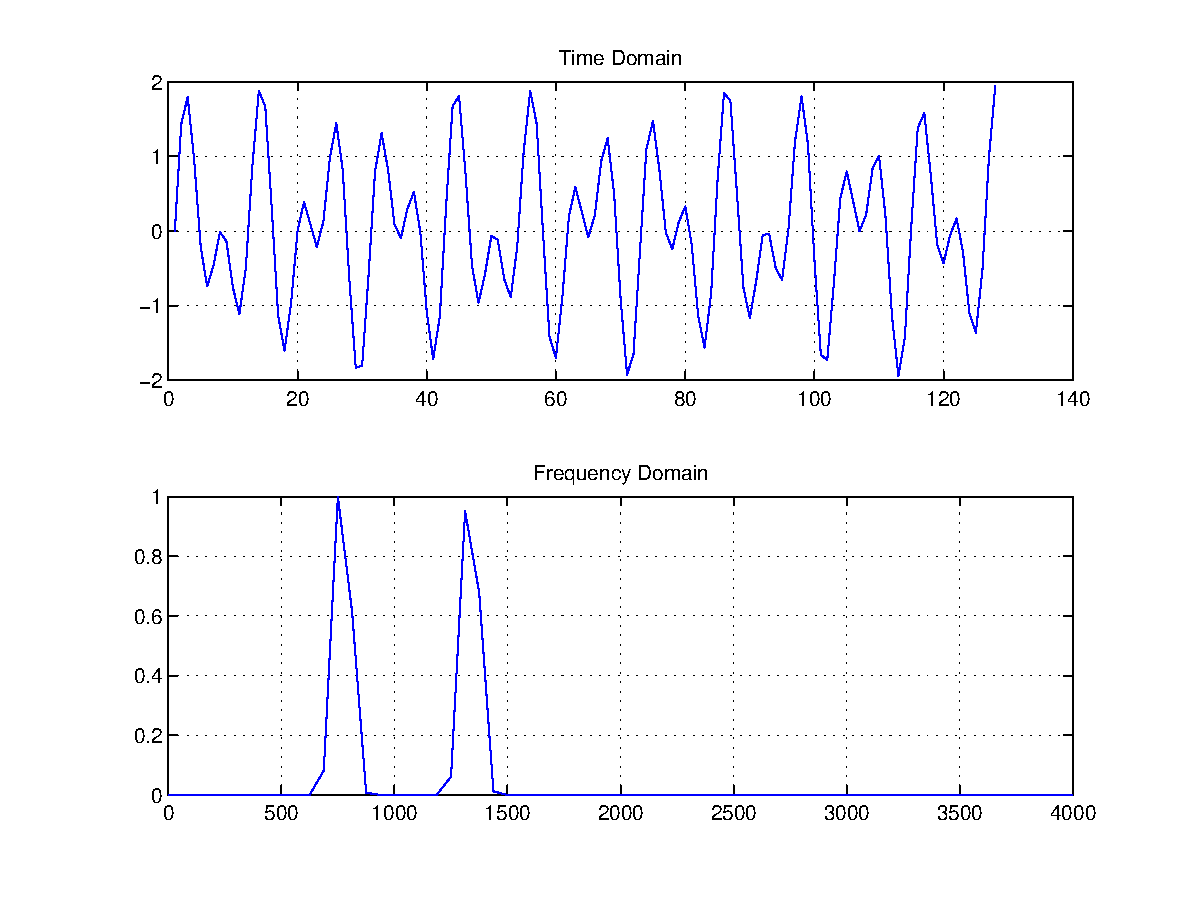
\includegraphics[width=2.5in]{./pic/dig5.eps}
 %\DeclareGraphicsExtensions.
\caption{Example FFT of dialing `5'}\label{fig:dail5}
\end{figure}
Once we can find the two peaks of the signal, the signal can be identified.

\subsection{Type I Chebyshev Filter}
\begin{figure}[!t]
\centering
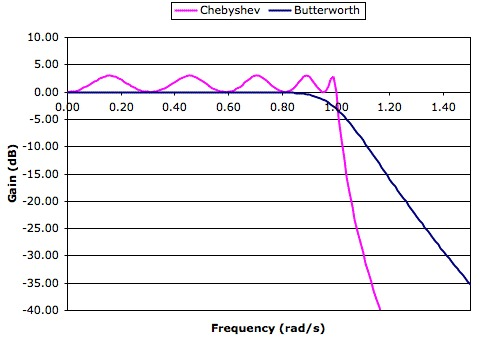
\includegraphics[width=2.5in]{./pic/cvb.jpg}
 %\DeclareGraphicsExtensions.
\caption{Compare of Filters}\label{fig:cvb}
\end{figure}
Chebyshev filters(Type I) are filters having a steeper roll-off and more passband ripple than the Butterworth filter(As shown in figure \ref{fig:cvb}). As in this application, there are frequencies need to be filtered but closed to the needed frequency(The highest busy tone is 620Hz and the lowest dial tone is 697Hz, only ~80Hz difference). So to minimize the error, we decided to choose Chebyshev filter rather than Butterworth filter in sacrificing of ripple in the passband.\\ 
\indent In addition, we only use the filter to identify frequency but not going to playback, the distortion in passband does not matter.


\section{Proposed Approach}
The decoder is accomplished following the flow chart in figure \ref{fig:fc}.\\
\tikzstyle{decision} = [diamond, draw, fill=blue!20, 
    text width=4.5em, text badly centered, node distance=3cm, inner sep=0pt]
\tikzstyle{block} = [rectangle, draw, fill=blue!20, 
    text width=8em, text centered, rounded corners, minimum height=3em]
\tikzstyle{line} = [draw, -latex']
\tikzstyle{cloud} = [draw, ellipse,fill=red!20, node distance=3cm,
    minimum height=2em]
\tikzstyle{clc} = [draw, circle,fill=red!20, node distance=3cm,
    minimum height=0.1]    
\begin{figure}
\centering
\begin{tikzpicture}[node distance = 2cm, auto,scale=0.6, every node/.style={transform shape}]
    % Place nodes
    \node [cloud] (file) {.wav file, "Method"};
    \node [block,below of=file,node distance=1.5cm](read){Read file  and method};
    \node [cloud,left of=read,node distance=5cm,text width=12em](f1){Function \\\scriptsize DTMFdecoder(`.wav file',`Method')};
    \node [block,below of=read,text width=15em,node distance=1.5cm](prefilter){690-1700Hz  Bandpass filter};
    \node [block,below of=prefilter,node distance=1.5cm](splitter){Digits\\Spliter};
    \node [decision,below of=splitter,node distance=2.5cm](loop){For every digits of the signal};
    \node [decision,below of=loop,node distance=3cm](method){Method};
    \node [cloud, below of=method,node distance=2cm](result){Result};
    \node [block, left of=result,node distance=3cm](fft){Decode Single Signal\\ Using FFT};
    \node [block, right of=result,node distance=3cm](filter){Decode Single Signal\\ Using Filter};
    \node [clc,below of=fft](ptm){};
    \node [left of=ptm](ptm2){};

    % Draw edges
    \path[line](file)--(read);
    %\path[line,dashed](read)--(f1);
    \path[line](read)--node{raw wave}(prefilter);
    \path[line](prefilter)--node{flitted wave}(splitter); 
    \path[line](splitter)--(loop);
     \path[line](loop)--node{position array}(method);
    \path[line](method)-|node[near end]{\scriptsize{Using FFT}}(fft);
    \path[line](method)-|node[near end]{\scriptsize{Using Filter}}(filter);
    \path[line](filter)--(result);
    \path[line](fft)--(result);
    \path[draw](filter)|-(ptm);
    \path[draw](fft)--(ptm);
    \path[draw](ptm)--(ptm2);
    \path[line](ptm2)|-(loop);

\end{tikzpicture}
\caption{Flow Chart for the decoder}
 \label{fig:fc}
\end{figure}
\subsection{Read file}
To read the wave file using Matlab, we use the commend:
\begin{lstlisting}
[RawWave,Fs]=wavread(WaveFile);%where WaveFile equals to the string of file name
\end{lstlisting}
Then we get the wave as a array in RawWave. In our occasion, we tested a real recored wave file `realrec1.wav' and get its wave form in figure \ref{fig:rwf} 
 \begin{figure}[!t]
\centering
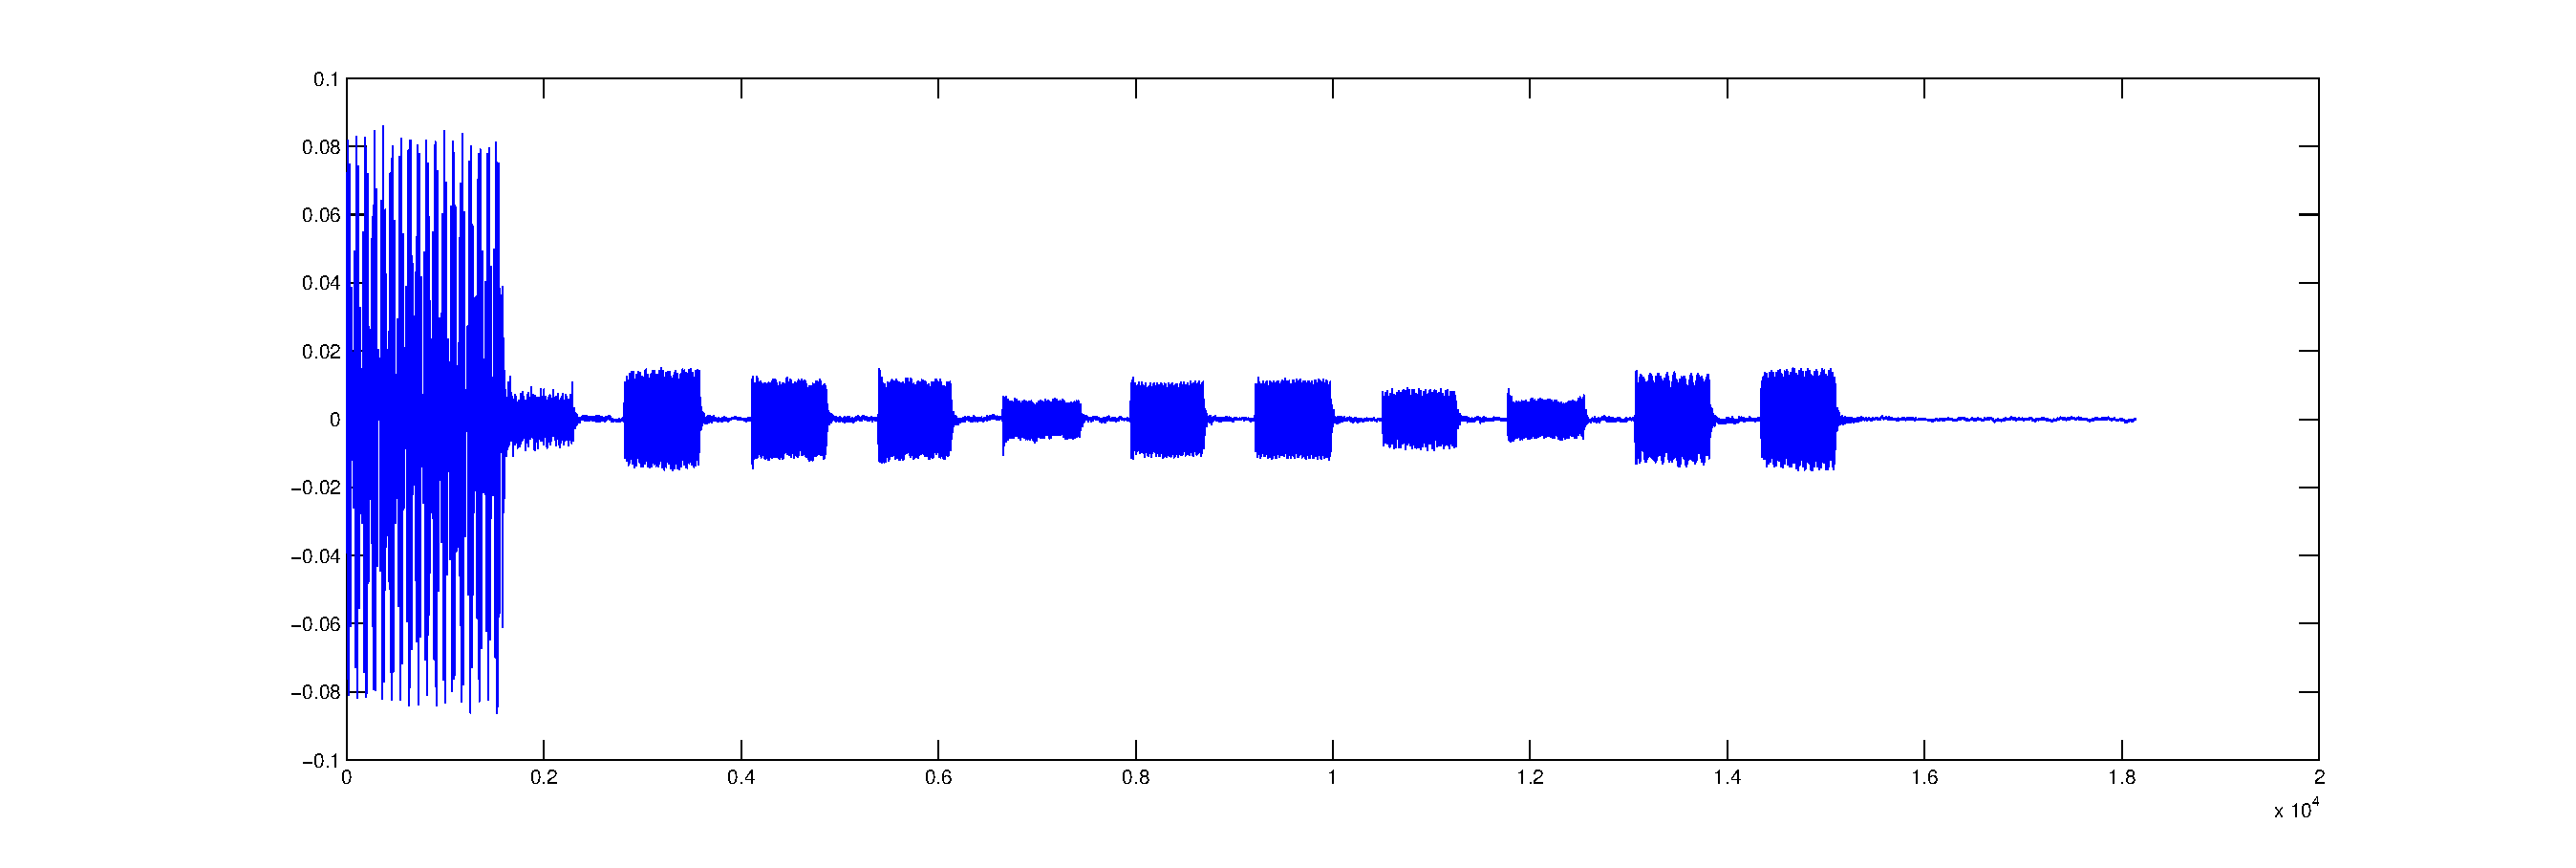
\includegraphics[width=0.5\textwidth]{./pic/RawWave.eps}
 %\DeclareGraphicsExtensions.
\caption{Waveform of Raw Input Wave}\label{fig:rwf}
\end{figure}

\subsection{Pre-filter}
From figure \ref{fig:rwf} we find that there exits lots of wave with large amplitude that we don't what and can cause trouble to wave analyze. So we need a band pass filter to get ride of them.\\
\indent Using the Matlab code:
\begin{lstlisting}
f1=680;f3=1700;
fsl=640;fsh=1740;
rp=0.1;rs=20;
wp1=2*pi*f1/Fs;
wp3=2*pi*f3/Fs;
wsl=2*pi*fsl/Fs;
wsh=2*pi*fsh/Fs;
wp=[wp1 wp3];
ws=[wsl wsh];
[n,wn]=cheb1ord(ws/pi,wp/pi,rp,rs);
[bz1,az1]=cheby1(n,rp,wp/pi);
FiltedWave=filter(bz1,az1,RawWave);
\end{lstlisting}
we get the Chebyshev filter in figure \ref{fig:pft}. 
 \begin{figure}[!t]
\centering
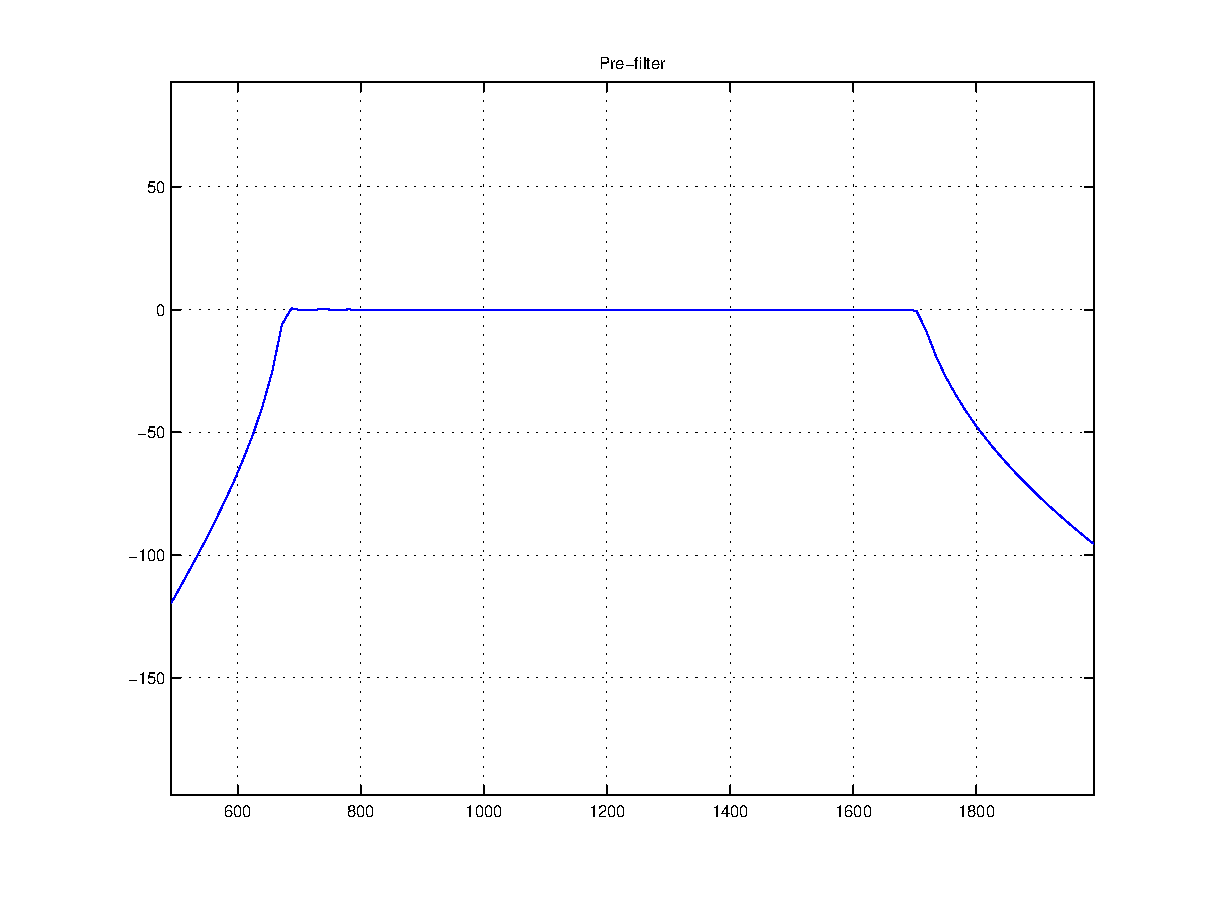
\includegraphics[width=0.5\textwidth]{./pic/pre_filter.eps}
 %\DeclareGraphicsExtensions.
\caption{Raw Wave After the Pre-filter}\label{fig:pft}
\end{figure}
Then the filtered wave will be cut off on the low frequency and the unnecessary high frequency, as shown in figure \ref{fig:ftw}.
 \begin{figure}[!t]
\centering
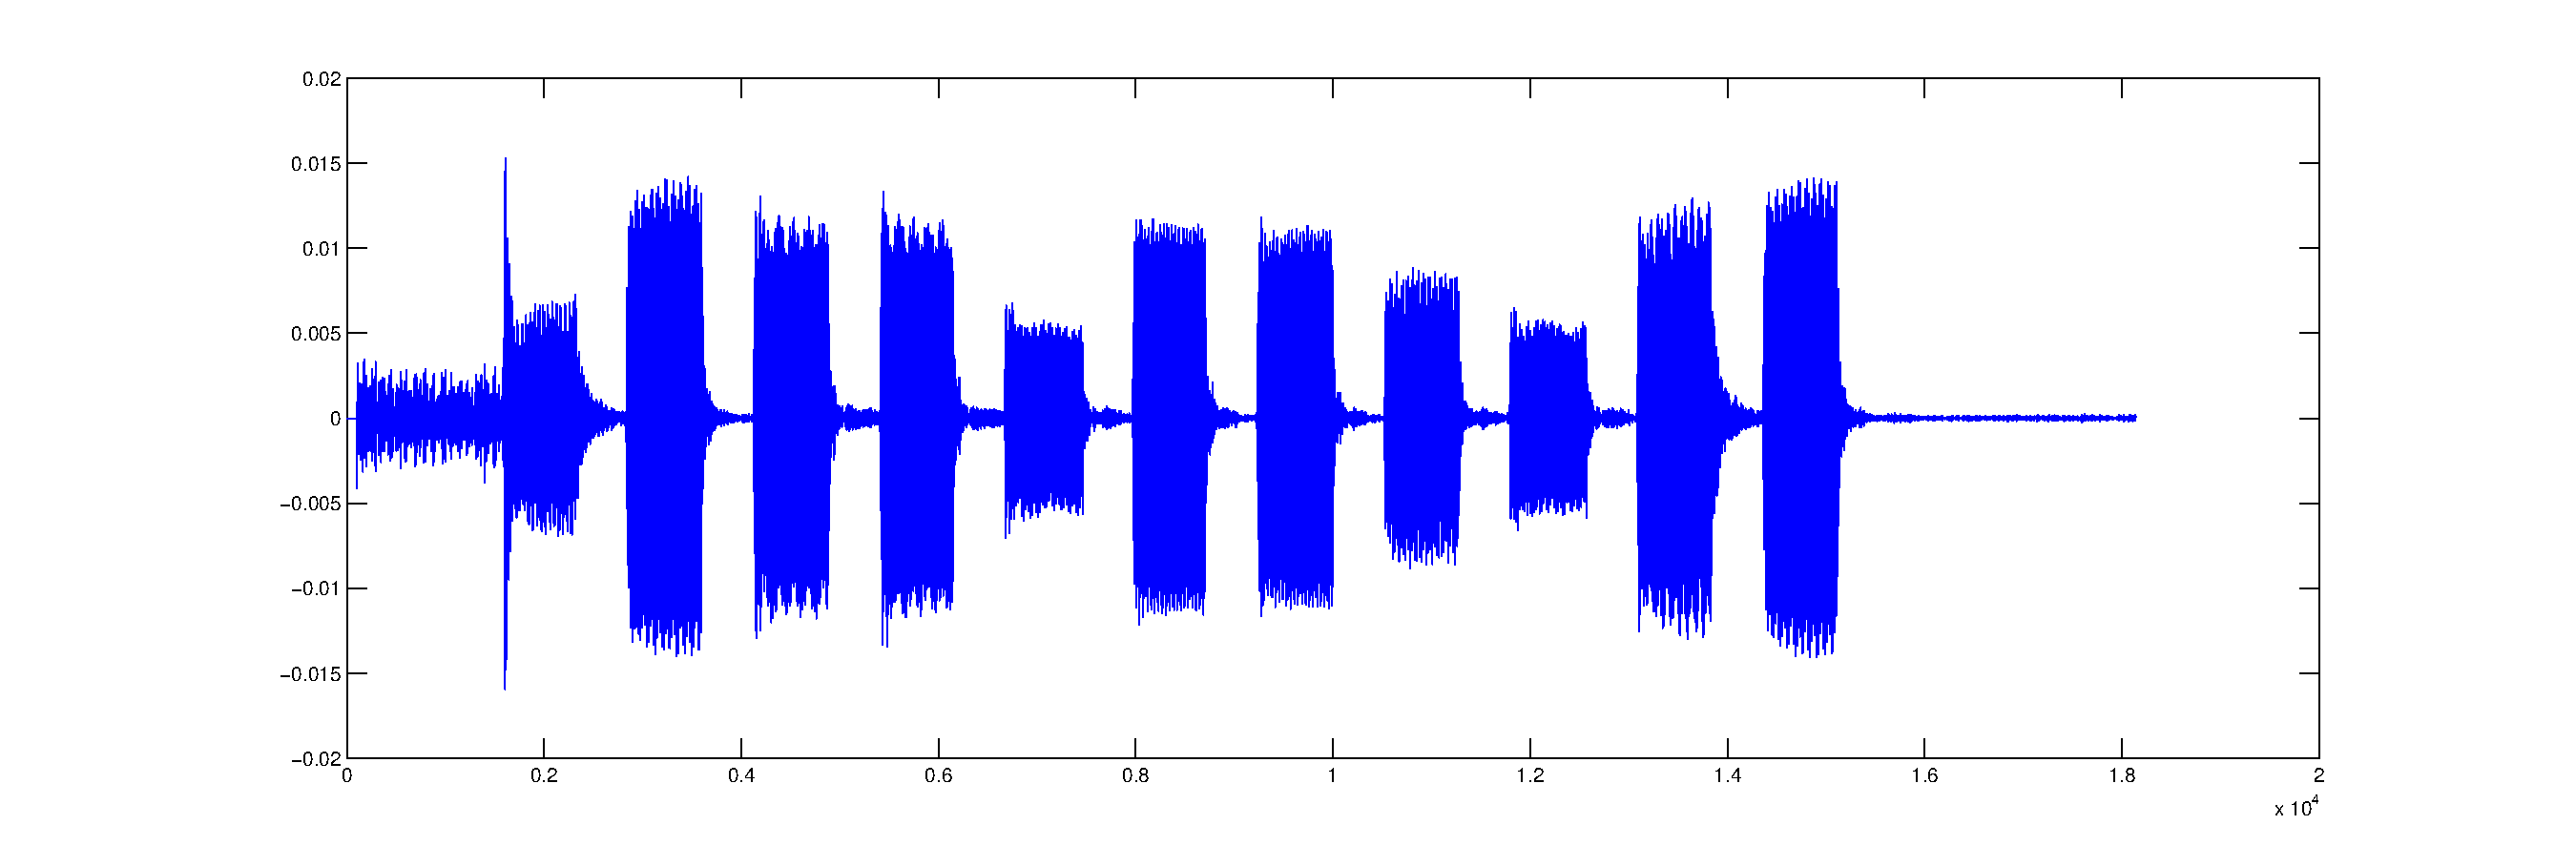
\includegraphics[width=0.5\textwidth]{./pic/FiltedWave.eps}
\caption{Pre-filter Frequency Response}\label{fig:ftw}
\end{figure}
\subsection{Split multi-digits}
	After we get the wave that only contains the frequencies components we want, we need to cut it into small, monotonous(or should be 'bitonous' here) pieces so that we can analyze them. To achieve this, we need a function `WaveSpliter', who takes in the raw wave and gives out an $n \times 2$ array that tell us where the dial tone starts and where it ends.\\
	\[
	PositionArray=
		\left(\begin{array}{cc}1st\ dial & 1st\ dial \\begin\ point & end\ point \\\vdots & \vdots \\\vdots & \vdots \\nth\ dial & nth\ dial \\begin\ point & end\ point\end{array}\right)
	\]
	To get this, we first find the envelope of the signals, as shown in figure \ref{fig:fwe}
\begin{figure}[!t]
\centering
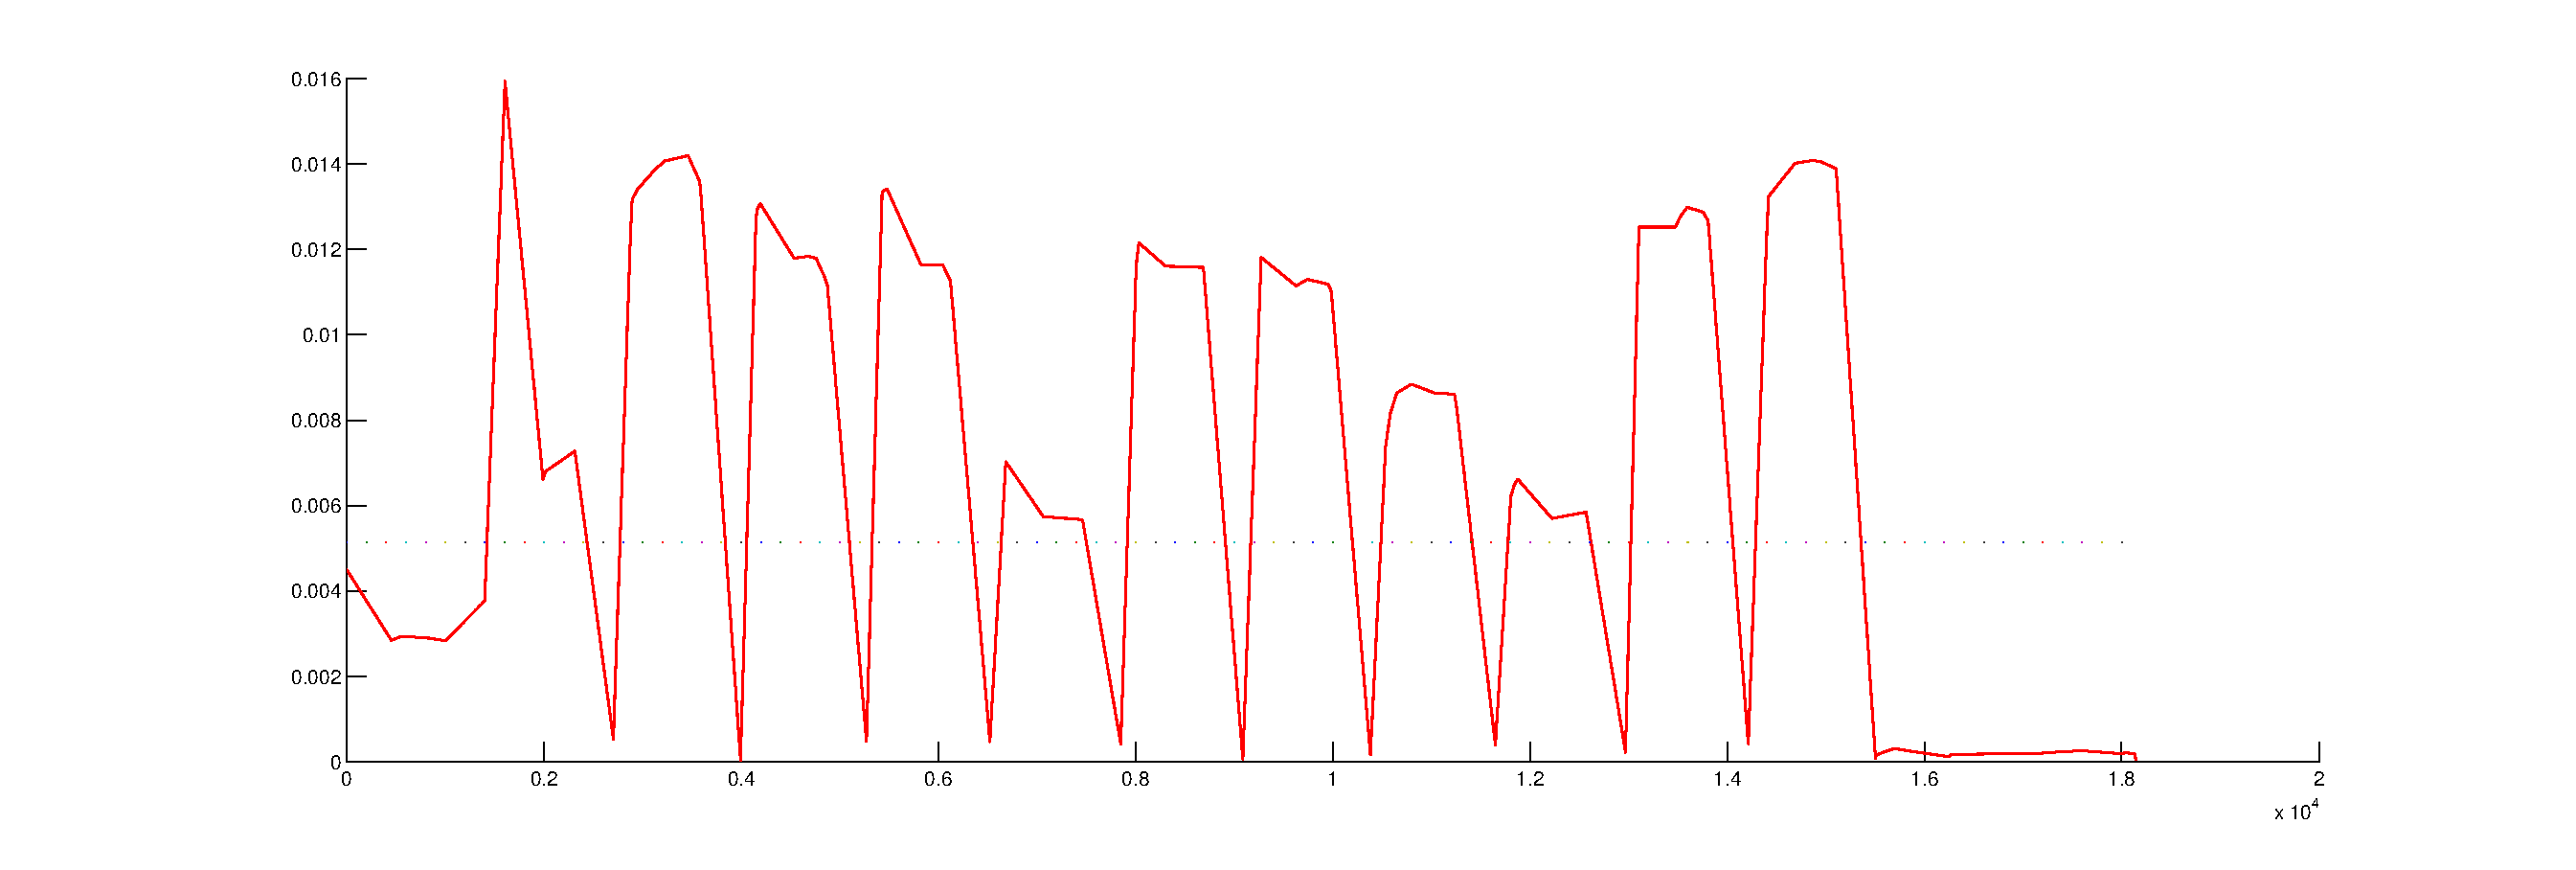
\includegraphics[width=0.5\textwidth]{./pic/FiltedWave_Env.eps}
\caption{Envelope of Filtered Raw Wave}\label{fig:fwe}
\end{figure}
Then we calculate the mean of the amplitude. Then scale it with proper value, here we divide it by 1.5, then take it like a threshold value. Find every point on the envelope that cross the threshold value, recored it as the beginning or end point of the dialing tone. 
\subsection{Decode Single Digits Using FFT}
Since we know where the monotonous signal begin and end, we can analyze them through different ways. The first way of approaching is to use FFT.\\
\indent The FFT of the signal will have two peaks, to identify them, we first need to filter the signal through two different filter, lowpass filter at 1000Hz and conjugating high pass filter, as shown in figure \ref{fig:fbf}. After this, we do FFT to the two signal, and now each signal in frequency domain should has only one peak. Now we can find the maximum of the function to find out the peak value and identify the signal. 
\begin{figure}
\centering
\subfigure[Lowpass Filter]{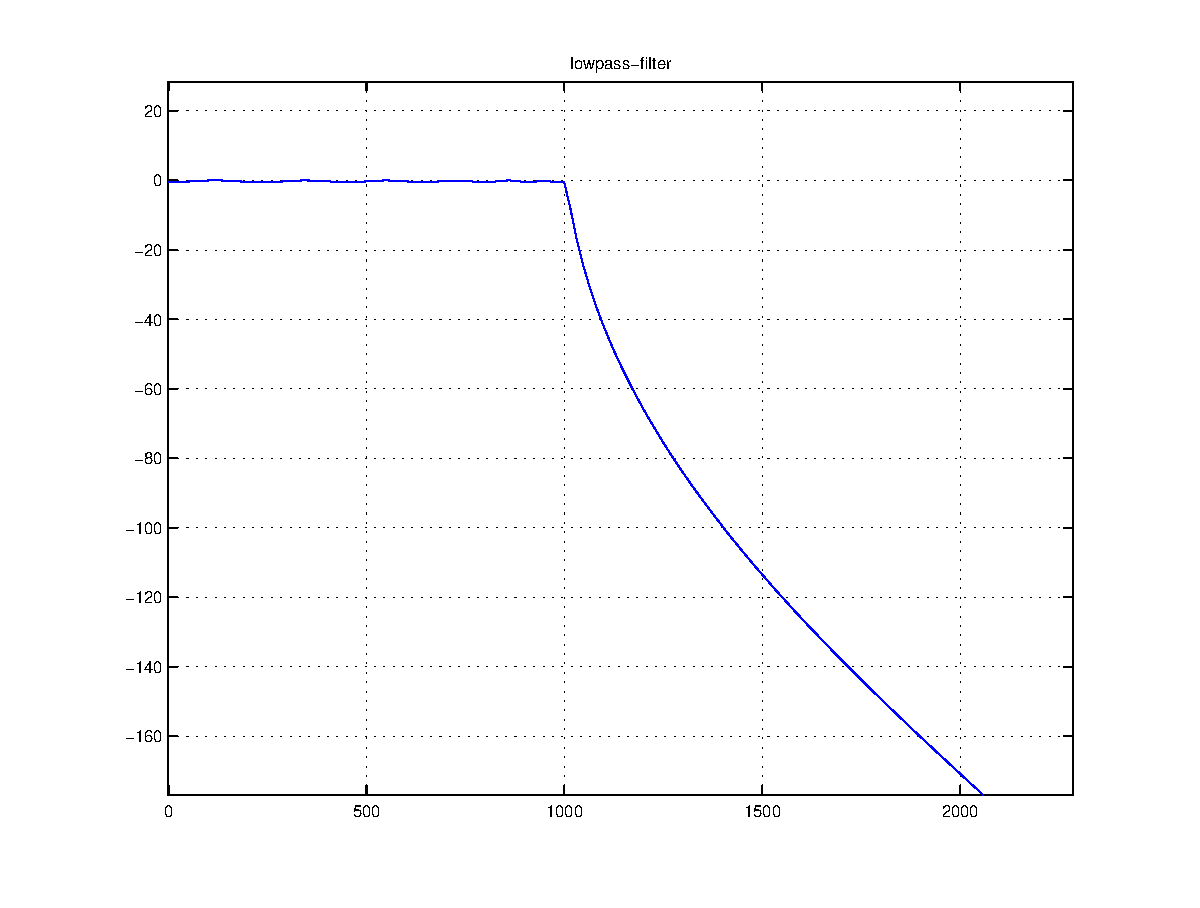
\includegraphics[width=0.45\textwidth]{./pic/lowpass.eps}}
%\mbox{\hspace{0.5cm}}
\\
\subfigure[Highpass Filter]{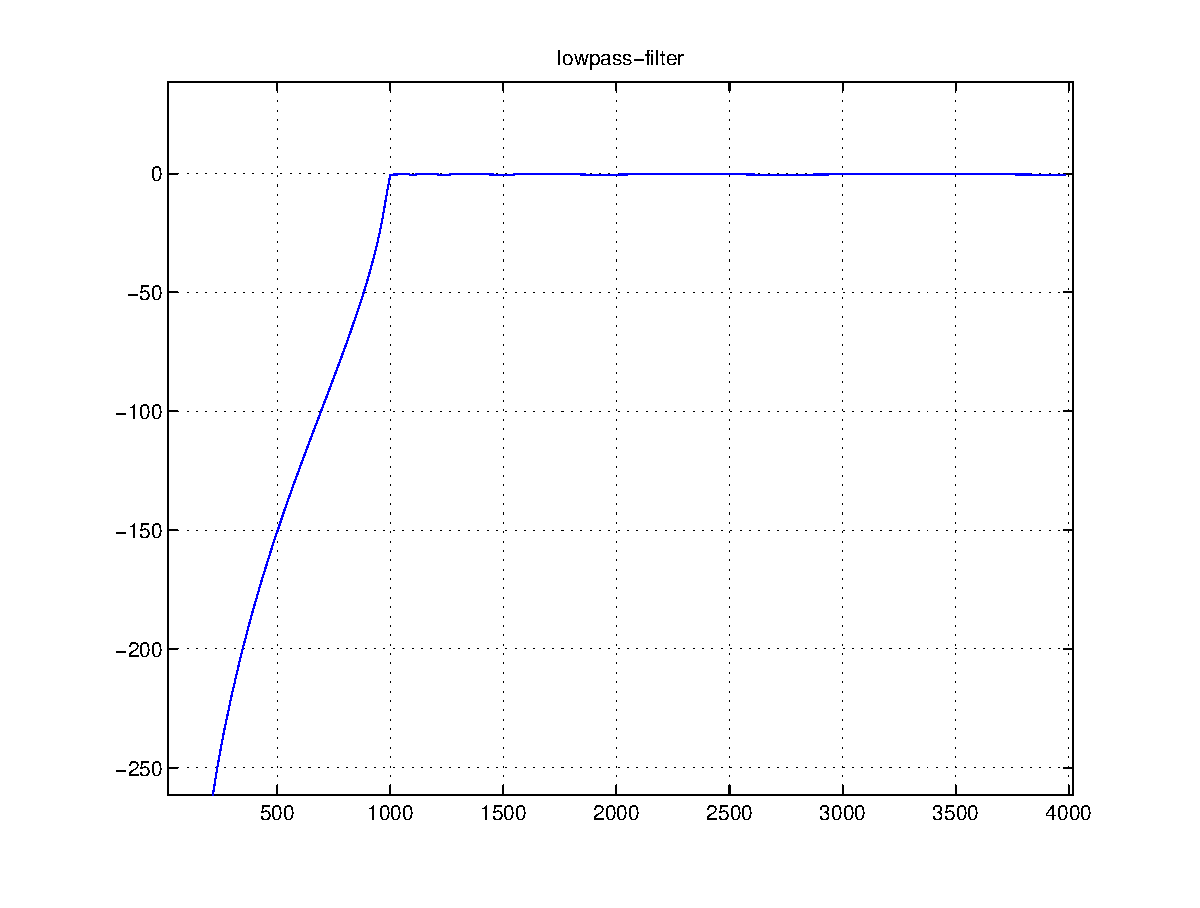
\includegraphics[width=0.45\textwidth]{./pic/highpass.eps}}
\renewcommand{\figurename}{Fig}
\caption{Filter Fefore FFT}
\label{fig:fbf}
\end{figure}
\subsection{Decode Single Digits Using Filter Bank}
For the filter bank approaching, we test the wave through two bandpass filter separately. There are 8 kind of filters, each of them can filter only one frequency of the DTMF and there are $4\times 4$ combinations. After the signal has passed through the two filter, we add the maximum of the two result signal. At last we will get 16 groups of maximum value, and the maximum of these maximum is the dial tone we want to decide. Figure \ref{fig:fb5} shows the occasion using filter band method to identify signal `5'
 \begin{figure}[!t]
\centering
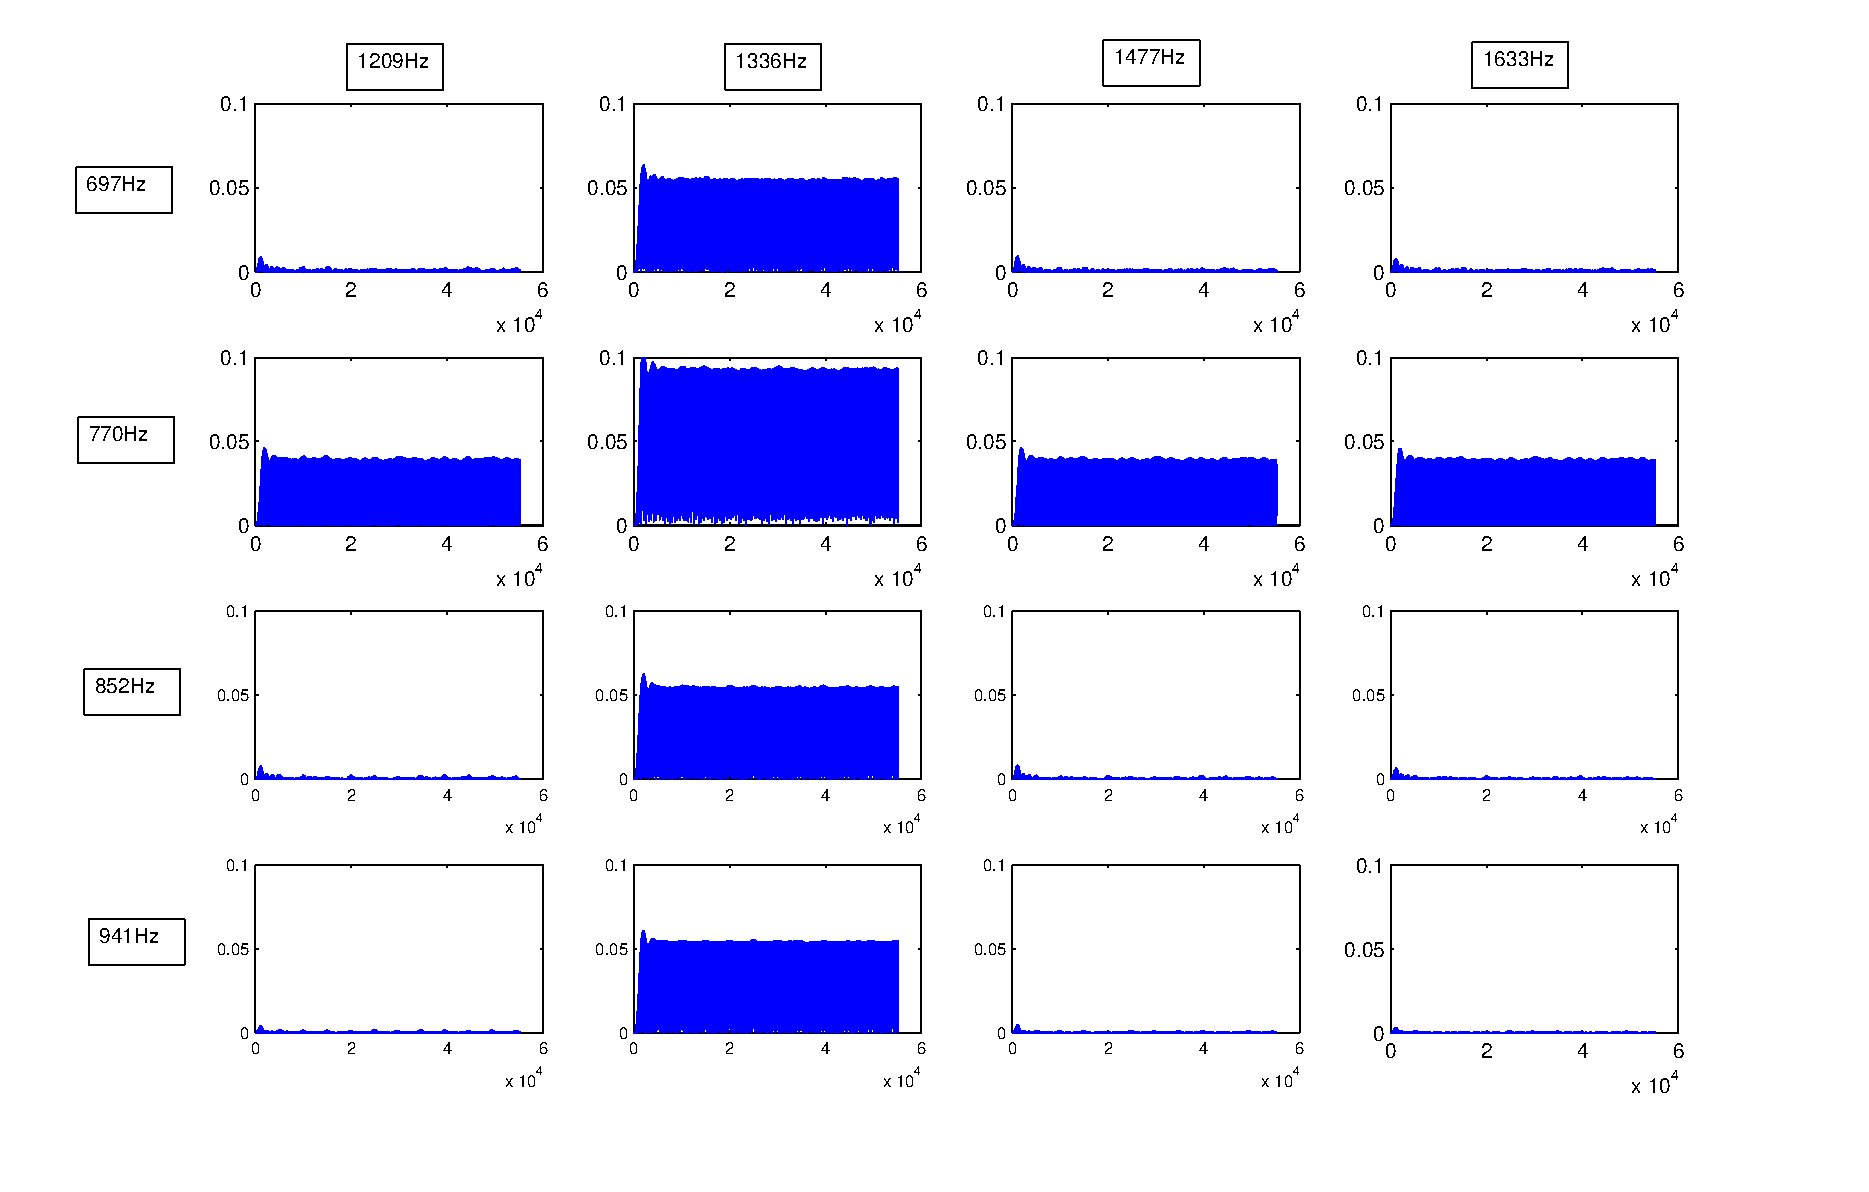
\includegraphics[width=0.5 \textwidth]{./pic/filterband5.eps}
\caption{Filter Band Identify Signal 5}\label{fig:fb5}
\end{figure}
\*\\
\section{Conclusion}
Finally we accomplished the function `DTMFdecoder'. It has two parameters, the inout wave file name and the methode string. The function can be used as:\\
\begin{lstlisting}
>>DTMFdecoder('realrec1.wav','FFT'); %for using FFT method to decode file realrec1.wav
>>DTMFdecoder('realrec1.wav','Filter'); %for using Filter method to decode file realrec1.wav
\end{lstlisting}
and the out put will be like:
\begin{lstlisting}
>> DTMFdecoder('realrec1.wav','FFT');%for using FFT method to decode file realrec1.wav
The code is 18664557438
>>DTMFdecoder('realrec1.wav','Filter'); %for using Filter method to decode file realrec1.wav
The code is 18664557438
\end{lstlisting}
Further, if the option 'graph' sets to 'gryphz\_on', the input wave will be played back and the waveform and the FFT of every digits will be shown, see figure \ref{fig:out}.
\begin{lstlisting}
>> DTMFdecoder('realrec1.wav','FFT','graph_on');
%for using FFT method to decode file realrec1.wav with graph on
The code is 18664557438
\end{lstlisting}
 \begin{figure}[!t]
\centering
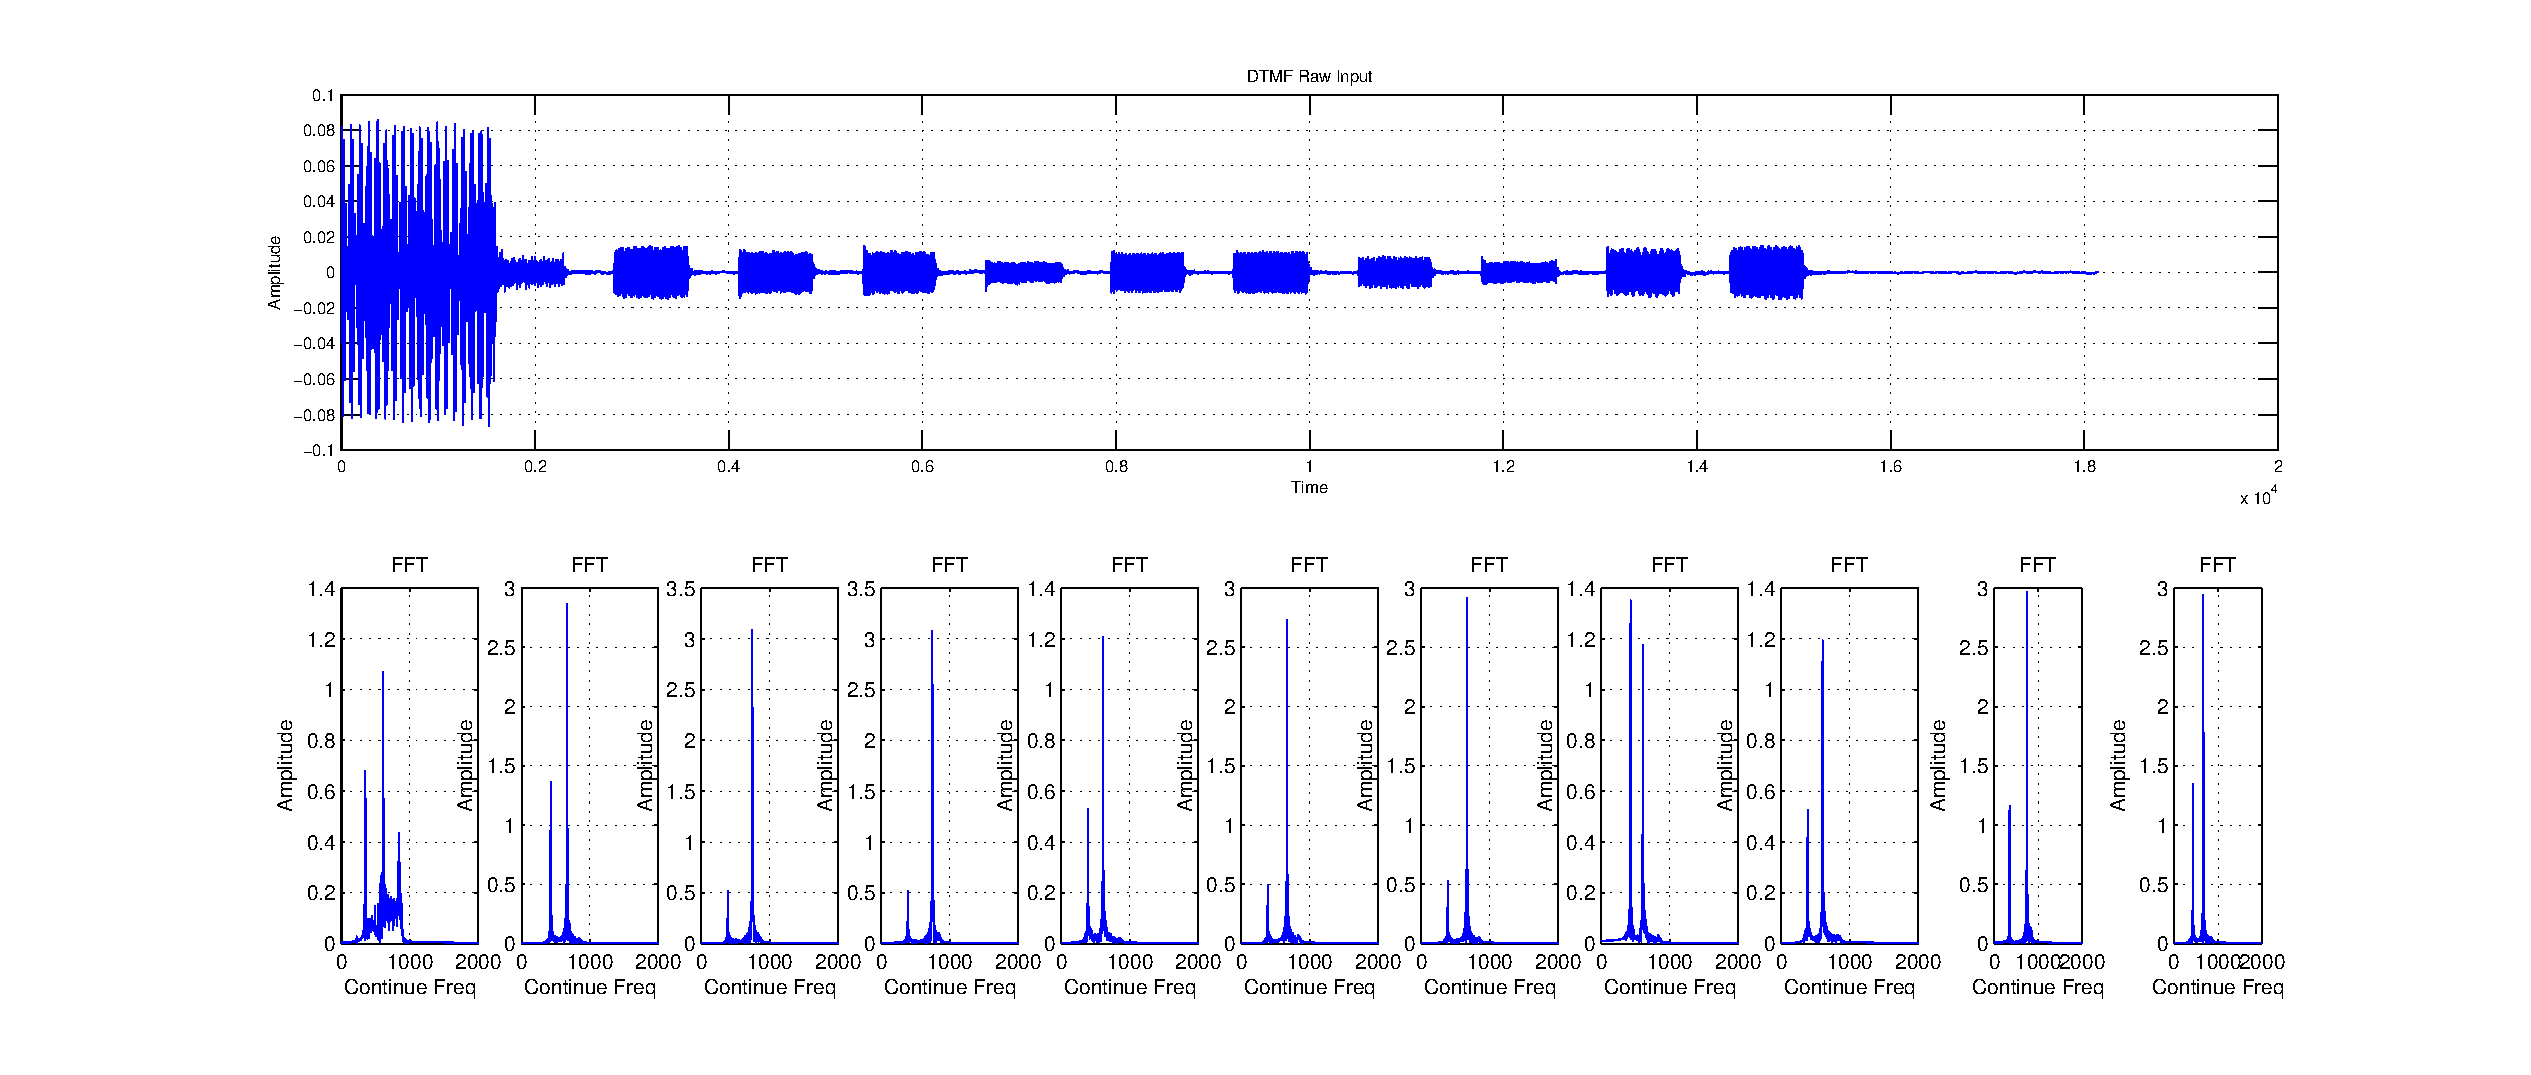
\includegraphics[width=0.5 \textwidth]{./pic/out.eps}
\caption{Filter Band Identify Signal 5}\label{fig:out}
\end{figure}

\appendices
\section{Code for the Whole Porject}
\subsection{DTMFdecoder.m}
\lstinputlisting[basicstyle=\ttfamily\tiny]{./MatlabCode/DTMFdecoder.m}
\subsection{WaveSpliter.m}
\lstinputlisting[basicstyle=\ttfamily\tiny]{./MatlabCode/WaveSpliter.m}
\subsection{envelope.m}
\lstinputlisting[basicstyle=\ttfamily\tiny]{./MatlabCode/envelope.m}
\subsection{DTMFdecoder\_single\_FFT.m}
\lstinputlisting[basicstyle=\ttfamily\tiny]{./MatlabCode/DTMFdecoder_single_FFT.m}
\subsection{DTMFdecoder\_single\_Filter.m}
\lstinputlisting[basicstyle=\ttfamily\tiny]{./MatlabCode/DTMFdecoder_single_Filter.m}
% you can choose not to have a title for an appendix
% if you want by leaving the argument blank

% use section* for acknowledgement
%\section*{Acknowledgment}
%
%
%The authors would like to thank...


% Can use something like this to put references on a page
% by themselves when using endfloat and the captionsoff option.
\ifCLASSOPTIONcaptionsoff
  \newpage
\fi



% trigger a \newpage just before the given reference
% number - used to balance the columns on the last page
% adjust value as needed - may need to be readjusted if
% the document is modified later
%\IEEEtriggeratref{8}
% The "triggered" command can be changed if desired:
%\IEEEtriggercmd{\enlargethispage{-5in}}

% references section

% can use a bibliography generated by BibTeX as a .bbl file
% BibTeX documentation can be easily obtained at:
% http://www.ctan.org/tex-archive/biblio/bibtex/contrib/doc/
% The IEEEtran BibTeX style support page is at:
% http://www.michaelshell.org/tex/ieeetran/bibtex/
%\bibliographystyle{IEEEtran}
% argument is your BibTeX string definitions and bibliography database(s)
%\bibliography{IEEEabrv,../bib/paper}
%
% <OR> manually copy in the resultant .bbl file
% set second argument of \begin to the number of references
% (used to reserve space for the reference number labels box)
\begin{thebibliography}{1}

\bibitem{bib:text}
A.~V.~Oppenheim and R.~W.~Schafer, \emph{Discrete-Time Signal Processing}, 3rd~ed.\hskip 1em plus
  0.5em minus 0.4em\relax Pearson Higher Education, Inc., Upper Saddle River: 2010.


\bibitem{bib:url}
bertrand.removethis.(2008,July,12) \emph{detect frequency of dtmf tone (.wav) file}, url={\url{http://compgroups.net/comp.soft-sys.matlab/detect-frequency-of-dtmf-tone-wav-file/957018}}.

\bibitem{bib:url}
bertrand.removethis.(2008,July,12) \emph{detect frequency of dtmf tone (.wav) file}, url={\url{http://compgroups.net/comp.soft-sys.matlab/detect-frequency-of-dtmf-tone-wav-file/957018}}.

\bibitem{bib:url}
Can Yi Tian Shi.(2011,Feb.,22) \emph{Sharing Matlab Program --- Filter}, url={\url{http://blog.sina.com.cn/s/blog_574d08530100qfrb.html}}.

\end{thebibliography}

% biography section
% 
% If you have an EPS/PDF photo (graphicx package needed) extra braces are
% needed around the contents of the optional argument to biography to prevent
% the LaTeX parser from getting confused when it sees the complicated
% \includegraphics command within an optional argument. (You could create
% your own custom macro containing the \includegraphics command to make things
% simpler here.)
%\begin{biography}[{\includegraphics[width=1in,height=1.25in,clip,keepaspectratio]{mshell}}]{Michael Shell}
% or if you just want to reserve a space for a photo:


% You can push biographies down or up by placing
% a \vfill before or after them. The appropriate
% use of \vfill depends on what kind of text is
% on the last page and whether or not the columns
% are being equalized.

%\vfill

% Can be used to pull up biographies so that the bottom of the last one
% is flush with the other column.
%\enlargethispage{-5in}



% that's all folks
\end{document}


